\subsection{DOM Engine\label{dom}}

The choice of DOM engine is central to the implementation.
We reviewed all major engines available today with respect to the requirements listed in \ref{design}:

The KDE Project's KHTML drives the Konquerer browser and some more exotic ones, but lacks a generic multi-platform build process.

This practical limitation is lifted by Apple's fork of KHTML, called WebKit.
It is the underlying engine of Safari browsers on Mac OS X and Windows. % and uses the JavaScriptCore.
There also exists a Qt and a GTK based open source implementation.
Whereas they are quite immature at the moment and not very widely used, this will change in the future and WepKit will certainly become a valuable option at some point.

Whereas the open source variant of Google's browser, \textit{Chromium}, promises superior execution speed by coupling WebKit with its own V8 JavaScript engine, it suffers from the same problem as WebKit itself namely, not being stable enough to serve as reliable platform --
the Linux client for example is barely usable, a Mac client does not even exist, yet.

We also briefly checked on Presto (Opera) and Trident (Microsoft), but discarded them due to their proprietary nature and lack of suitable APIs.

The Gecko engine (Mozilla Corporation) in conjunction with its JavaScript implementation Spidermonkey marks a special case:
It implements XUL \cite{xul}, the XML User Interface Language, as a way to create feature rich cross-platform applications.
The most prominent of those is the Firefox browser, but also e.g. Thunderbird, Sunbird and Flock are built with XUL.
An add-on system is provided that allows extending the functionality of XUL applications to third-party code that gains full access to the DOM representation, including the XUL part itself.
The proposed {\KrdWrd} back-end can be implemented in the same manner as Firefox: provide custom JavaScript and XUL code on top of Mozilla's core XUL Runner. 
Code can easily be shared between a browser add-on and XUL applications and unsupervised operation is trivial to implement in a XUL program.

Given the synergy attainable in the XUL approach and Firefox' popularity amongst users, it was a simple decision to go with Mozilla Gecko for the core DOM implementation.
We note that WebKit's rise and fast pace of development might change that picture in the future.

\subsubsection{Firefox Add-on}

Interactive visual annotation of corpus pages via Web browser is realized by the {\KrdWrd} Firefox add-on.
To facilitate adoption, it comes with a comprehensive user manual and an interactive tutorial (see below in \ref{webs}).
For easy setup, Firefox' proxy configuration is automatically pointed to a preconfigured host, respective credentials are auto-added to the password manager and the user is directed to a special landing page upon successful installation.
The proxy feature also serves as a nice example of code shared between add-on and application.
Furthermore, the installation binary is digitally signed, so the user does not have to go through various exception dialogs.


Once installed, the functionality of the Add-on is available via a broom icon in the status bar.
Whereas it offers lots of functions centered around annotation and corpus selection, its core feature is simple:
In highlight mode (the broom turns fuchsia) the mouse hovering over the page will highlight the text blocks below the cursor.
The block can then be annotated using the context-menu or a keyboard short-cut, which will change its color to the one corresponding to the annotation class.
Figure \ref{f:tut0} shows a fully annotated page and the context-menu.

\begin{figure}
\jss{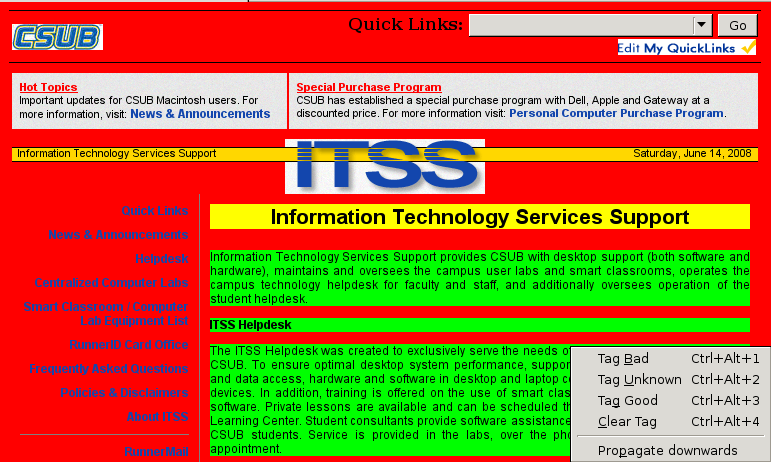
\includegraphics[width=0.5\textwidth]{tut0}}
	{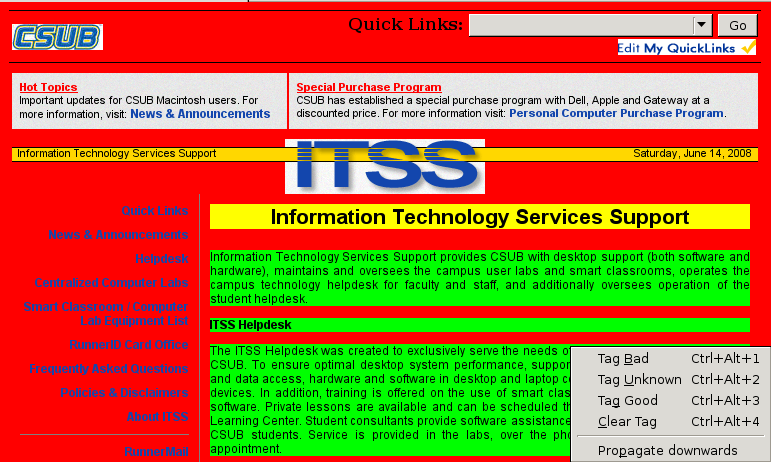
\includegraphics[width=0.8\textwidth]{tut0}}
\caption{\label{f:tut0}Web pages can be annotated with the {\KrdWrd} Firefox Add-on by hovering over the text by mouse and setting class labels by keyboard short-cut or pop-up menu.}
\end{figure}


\subsubsection{XUL Application \label{app}}

The XUL application consists of a thin JavaScript layer on top of Mozilla's XUL Runner.
It mainly uses the XUL browser control to load and render Web pages and hooks into its event handlers to catch completed page load events and the-like.
Without greater C level patching, XUL still needs to create a window for all of its features to work.
In server applications, we suggest using a virtual display such as Xvfb to fulfil this requirement.

In operation the application parses the command-line given, which triggers the loading of supplied URLs (local or remote) in dedicated browser widgets.
When the ``load complete'' event fires, one of several extraction routines is run and results are written back to disk.
The implemented extraction routines are 
\begin{description}
\item[grab] for simple HTML dumps and screen-shots,
\item[diff] for computing a visual difference rendering of two annotation vectors for the same page,
\item[merge\label{merge}] for merging different annotations on the same Web page into one in a simple voting scheme, and
\item[pipe] for textual, structural and visual data for the feature pipelines.
\end{description}

\subsection{Storage and Control\label{server}}

Central storage of Web pages and annotation data is provided by a database.
Clients access it via CGI scripts executed by a Web server while the back-end uses python wrapper scripts for data exchange.

\subsubsection{Web Server\label{webs}}

Server-side logic is implemented by Python CGI scripts, so any Web server capable of serving static files and executing CGI scripts is supported.
Users can access the server directly by URL or via the Firefox Add-on menu.
An overview page rendered by the server provides a submission overview as well as a detailed per-corpus submission list.
In conjunction with the Add-on, server side scripts control serving of corpus pages by summing over submissions in the database and randomly selecting a page from those with the least total submission number.
The Web server also delivers the actual HTML data to the client, whereas any embedded objects are served by the separate proxy server.
Furthermore, it controls the tutorial: Users are presented with sample pages and asked to annotate them.
Upon submission, a server side script compares the user's annotation with a reference annotation stored in the database and generates a page that highlights differences.
The result is delivered back to the user's browser as seen in figure \ref{f:tut1}.

\begin{figure}
\jss{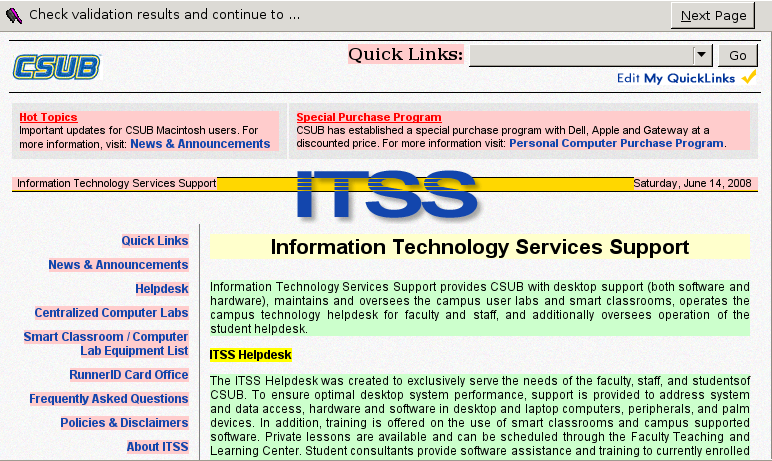
\includegraphics[width=0.5\textwidth]{tut1}}
	{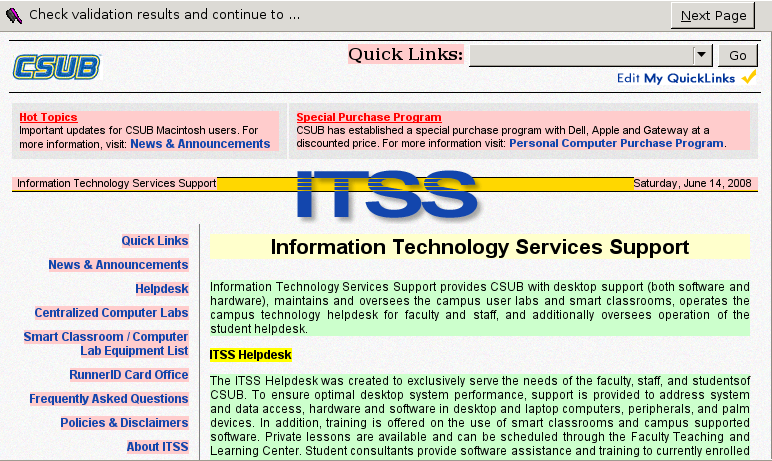
\includegraphics[width=0.8\textwidth]{tut1}}
\caption{\label{f:tut1}During the tutorial, a Visual Diff between the user's submission and the sample data is presented right after submission.
	Here, the annotation from \ref{f:tut0} was wrong in tagging the sub-heading ``ITSS Helpdesk'': the correct annotation (\textit{yellow}) is highlighted in the feedback.}
\end{figure}

\subsubsection{Database}

The database mainly stores the raw HTML code of the corpus pages.
User submissions are vectors of annotation classes, the same length as the number of text nodes in a page.
In addition there is a user mapping table that links internal user ids to external authentication.
Thereby user submissions are anonymized, yet trackable by id.

Given the simple structure of the database model, we choose to use zero-conf database back-end \textit{sqlite}.
This should scale up to some thousand corpus pages and users.

It is important to note that any database content must be pre-processed to be encoded in UTF-8 only.
Unifying this bit of data representation at the very start is essential to avoid \textit{encoding hell} later in the process.
\subsubsection{Proxy}

Any object contained in the corpus pages needs to be stored and made available to viewers of the page without relying on the original Internet source.

Given an URL list, initial population of the proxy data can easily be achieved by running the XUL application in grabbing mode while letting the proxy fetch external data.
Afterwards, it can be switched to block that access, essentially creating a closed system.
We found WWWOffle to be a suitable proxy with support for those features while still being easy to setup and maintain.

\subsection{Feature Extractors\label{extract}}

The XUL Application extracts information from corpus pages and dumps it into the file-system, to serve as input to specialized feature extractors.
This implementation focuses on feature extraction on those nodes carrying textual content, providing one feature vector per such node.
We therefore generate one feature vector per such node through a linguistic, visual and DOM-tree focused pipeline.

\subsubsection{Text}

For linguistic processing, the Application dumps raw text from the individual nodes, with leading and trailing whitespace removed, converted to UTF-8 where applicable.
External applications can read these data and write back the feature vector resulting from their computation in the same format.

\subsubsection{Structural}

During an Application run, a set of ``DOM-Features'' is directly generated and dumped as feature vector.

Choosing the right DOM properties and apply the right scaling is a non-trivial per-application decision.
Our reference implementation includes features such as depth in the DOM-tree, number of neighboring nodes, ratio text characters to HTML code characters,
  and some generic document properties as number of links, images, embedded objects and anchors.
We also provide a list of the types of node preceding the current node in the DOM-tree.


\subsubsection{Visual}

\begin{figure}

\includegraphics[width=0.5\textwidth]{vizwrap}
\caption{\label{f:vizwrap}Coordinates of a node's bounding box (straight) and text constituents (dotted) as provided to the visual processing pipeline.}
\end{figure}

For visual analysis, the Application provides full-document screen-shots and coordinates of the bounding rectangles of all text nodes.%
\footnote{This Extractor requires at least XUL Runner Version 1.9.2 (corresponding to Firefox Version 3.5) which is still in beta at the time of this writing.}
When text is not rendered in one straight line, multiple bounding boxes are provided as seen in figure \ref{f:vizwrap}.
This input can be processed by any application suitable for visual feature extraction.

For simple statistics dealing with the coordinates of the bounding boxes, we use a simple Python script to generate basic features such as total area covered in pixel, number of text constituents, their variance in x-coordinates, average height and the-like.

Furthermore, we provide a tool chain to use the JAMF framework \cite{Steger08}, a component-based client/server system for building and simulating visual attention models.
The ``CoordRect'' JAMF component generates masks the same size as the Web page screen-shot based on the node coordinates.
It therefore allows region-wise analysis of the page rendering with the default component set provided by JAMF, which is focused on visual feature extraction.
Results are read by the JAMF Python client and converted into feature vectors on a per-node basis.

Clearly, the components and filter of JAMF model employed or using an entirely different framework for actually visual feature extraction are per-application decisions to be made.


